% L10c Thompson sampling figure: the two posteriors of the lecture's worked
% example and the one sample drawn from each.
%
% Drawn on October 21, 2026 with the palette and build of the L10c bandit arms
% figure.
%
% Each arm is a row on a success-probability scale (11 cm per unit) with its
% posterior density drawn above the row (0.45 cm per unit density). With uniform
% Beta(1, 1) priors, the posteriors, normalizing constants 1/B(a, b), and means
% are:
%   arm 1: 3 successes, 1 failure, Beta(4, 2), 20, mean 2/3
%   arm 2: 0 successes, 1 failure, Beta(1, 2),  2, mean 1/3
% The tick at each mean runs from the row to the density. The dot is the
% arm's posterior sample: p(1) = 0.55 and p(2) = 0.70. Arm 2 has the larger
% sample, so Thompson sampling pulls it, although its mean is lower.
%
% Labels are set large so they stay readable when the slide scales the figure
% down. Math uses the standard TeX fonts (no unicode-math), so symbols render as the
% notebook's math shows them.
%
% The notebook SVG carries a dark palette added by theme_svg.py; keep new
% colors in that script's mapping when changing the palette here.
\documentclass[tikz,border=4pt]{standalone}
\usepackage[no-math]{fontspec}
\IfFontExistsTF{Arial}{\setsansfont{Arial}}{\setsansfont{TeX Gyre Heros}}
\renewcommand{\familydefault}{\sfdefault}
\usepackage{amsmath,amssymb}

% Ink, blue, gray, and the two fills match the bandit arms figure; blue marks
% the selected arm.
\definecolor{vnink}{HTML}{202124}
\definecolor{gdblue}{HTML}{0091FF}
\definecolor{gdgray}{HTML}{6D7278}
\definecolor{waband}{HTML}{EEF0F2}
\definecolor{bafill}{HTML}{B3DCFF}

% \posterior{row y}{alpha}{beta}{1/B(alpha, beta)}{fill}{edge}: a Beta density
% drawn above a horizontal success-probability row.
\newcommand{\posterior}[6]{%
  \filldraw[fill=#5, draw=#6, line width=0.8pt]
    plot[domain=0:1, samples=201]
      ({11*\x}, {#1 + 0.45*#4*(\x)^(#2 - 1)*(1 - \x)^(#3 - 1)}) -- (11, #1) -- (0, #1) -- cycle;}
% \meantick{row y}{alpha}{beta}{1/B(alpha, beta)}{mean}: the posterior mean, a
% tick from the row to the edge of the density.
\newcommand{\meantick}[5]{%
  \pgfmathsetmacro{\h}{0.45*#4*(#5)^(#2 - 1)*(1 - #5)^(#3 - 1)}
  \draw[vnink, line width=1.2pt] (11*#5, #1) -- (11*#5, #1 + \h);}

\begin{document}
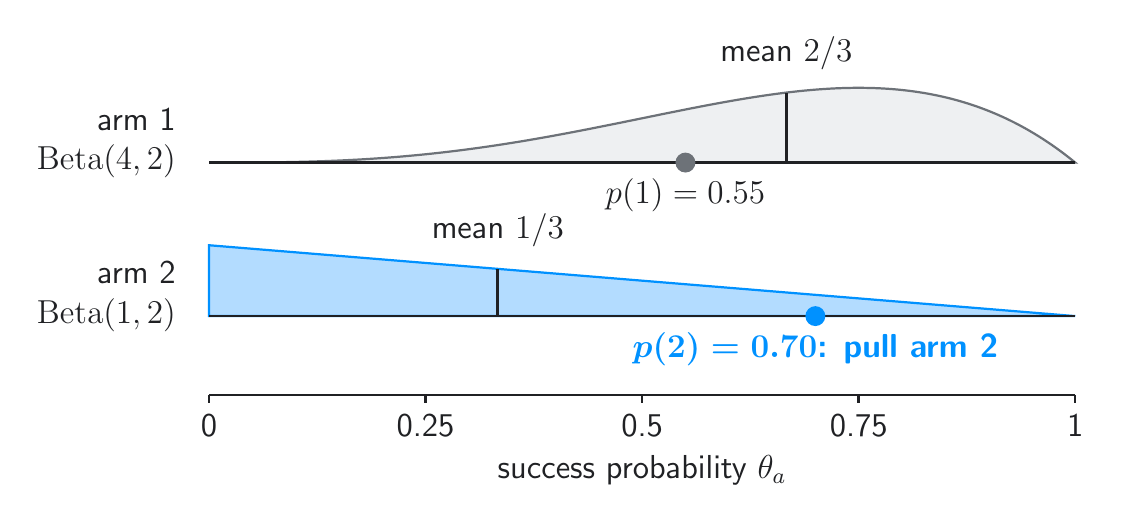
\begin{tikzpicture}[x=1cm, y=1cm, font=\sffamily\large, text=vnink,
    cell/.style={text height=1.6ex, text depth=0.45ex},
  ]
  % arm 1: Beta(4, 2), mean 2/3, sample 0.55
  \posterior{0}{4}{2}{20}{waband}{gdgray}
  \meantick{0}{4}{2}{20}{0.6667}
  \draw[vnink, line width=0.9pt] (0, 0) -- (11, 0);
  \node[cell, anchor=east] at (-0.3, 0.5) {arm 1};
  \node[cell, anchor=east] at (-0.3, 0) {$\mathrm{Beta}(4,2)$};
  \node[anchor=south] at (7.333, 1.05) {mean $2/3$};
  \fill[gdgray] (6.05, 0) circle (3.6pt);
  \node[cell, anchor=north] at (6.05, -0.15) {$p(1)=0.55$};

  % arm 2: Beta(1, 2), mean 1/3, sample 0.70; the larger sample, so it is pulled
  \posterior{-1.95}{1}{2}{2}{bafill}{gdblue}
  \meantick{-1.95}{1}{2}{2}{0.3333}
  \draw[vnink, line width=0.9pt] (0, -1.95) -- (11, -1.95);
  \node[cell, anchor=east] at (-0.3, -1.45) {arm 2};
  \node[cell, anchor=east] at (-0.3, -1.95) {$\mathrm{Beta}(1,2)$};
  \node[anchor=south] at (3.667, -1.2) {mean $1/3$};
  \fill[gdblue] (7.7, -1.95) circle (3.6pt);
  \node[cell, anchor=north, text=gdblue, font=\sffamily\large\bfseries] at (7.7, -2.1) {$\boldsymbol{p(2)=0.70}$: pull arm 2};

  % success-probability scale
  \draw[vnink, line width=0.9pt] (0, -2.95) -- (11, -2.95);
  \foreach \v in {0, 0.25, 0.5, 0.75, 1} {
    \draw[vnink, line width=0.9pt] (11*\v, -2.95) -- (11*\v, -3.05);
    \node[cell, anchor=north] at (11*\v, -3.1) {\v};
  }
  \node[anchor=north] at (5.5, -3.6) {success probability $\theta_a$};
\end{tikzpicture}
\end{document}
